%

\documentclass[10pt,article]{article}
\usepackage[T1]{fontenc}
\usepackage[utf8]{inputenc}
\usepackage{graphicx}
\usepackage{hyperref}
\usepackage[font={small,it}]{caption}
\usepackage[a4paper,top=1.1cm,bottom=2cm,left=1.9cm,right=1.9cm]{geometry}
\usepackage{color, colortbl}
\usepackage{tabularx}
\usepackage{sectsty}
\usepackage{hyperref}
\definecolor{Gray}{gray}{0.85}
\sectionfont{\huge}
\renewcommand{\familydefault}{\sfdefault}
\captionsetup{labelfont=bf}

\title{LUMS Stepper -- universal 3-axis stepper motor controller}
\author{Kacper Oreszczuk}
\date{}
\begin{document}

\maketitle
\section{Motivation}
Stepper motors are commonly used in laboratory. They are powering x-y-z translation stages, tunable filters, polarisation optics and many other devices. The goal of this project is to replace commercially available drivers with a cheaper, more reliable and more universal solution. 

\subsection*{Cost:}
Commercially available stepper motor drivers designed for laboratory use can reach prices
of a few hundred US\ Dollars for a single axis. Proposed solution costs about \$30 per axis with small
labour cost.

\subsection*{Quality:}
Personal experience in our laboratory revealed problems with microstep precision in drivers supplied by one of the leading laboratory equipment manufacturers. I have tested thoroughly stepper motor chip before choosing it for this project. 
\subsection*{Features:}
Custom solution allowed me to implement important additional features. The most important is automatic compensation of mechanical hysteresis.

\section{Hardware design}

Single device is able to control three bipolar stepper motors with 1/64 microsteps precision. Maximum current is about \SI{1.5}{A} per motor and the supply voltage must be between \SI{6}{V} and \SI{30}{V}.
Low level motor driving operation  is performed by\textit{AMIS-30543} driver on \textit{Pololu} breakout board. Three such drivers are connected to \textit{NUCLEO32}  board with \textit{STM32L432KC} microcontroller. Nucleo board connected via USB to computer provides virtual serial port for communication and power for logic layer of device. Separate power connector is provided on main PCB for motor operation and three high-density D-SUB15 female connectors (ICD15S13E4GV00LF) for motors. Full schematics of the device is presented in Figure \ref{schematics}. PCB board is double-sided. See Figure \ref{pcb} for PCB layout. This design, which effectively consists of 8 elements makes the project easy and quick to deploy in several copies. The driver is confined in 3D-printed case (Figure \ref{case}) protecting it and allowing mounting to optic table. Picture \ref{photo} shows assembled device with the top lid removed. Design files for PCB and case along with source code for microcontroller are available at project page: \url{github.com/kacperoreszczuk/lums_stepper/}. 

\begin{figure}[h]
 \centering
 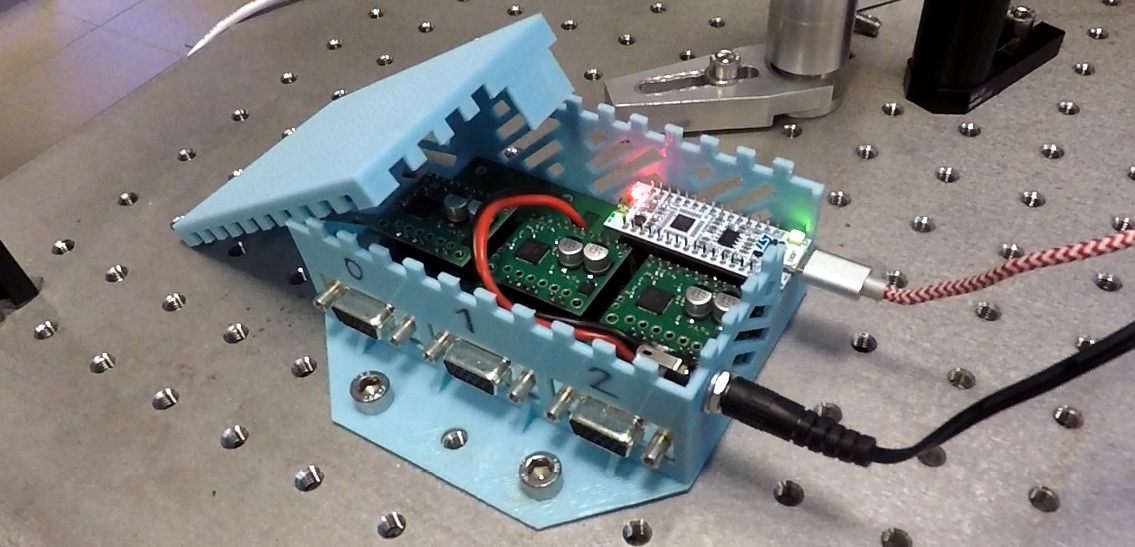
\includegraphics[width = 11.5cm]{photo.png}
\caption {Assembled LUMS Stepper.} \label{photo}
\end{figure}
\newpage
\section{Software and protocol}

Driver has two basic operation modes - movement with given velocity or movement to given position. In either of the cases the movement of motor is smoothed at starting and stopping. For user convenience speeds and positions are expressed in real units (for example millimeters in case of linear travel stage), not motor steps. End switches (limit switches) of different types are supported by this driver. They provide additional safety, as the driver will stop at the edge of the movement range of, for example, linear translation stage. Limit switches are also used to automatically calibrate absolute position of the stage.

When the mechanical setup of driven actuator is not completely rigid, the mechanical hysteresis can occur. Due to this effect real position of the  actuator depends on the direction from which set position is approached. In this project user can specify the amplitude od mechanical hysteresis. Algorithm will track previous movements and compensate the offsets in a manner transparent for the user.  

User can communicate with LUMS Stepper via virtual serial port provided by Nucleo board. Protocol of communication is based on single line plain-text commands initiated from computer and on single line reply from driver. For protocol description please refer to Table \ref{protocol}. Full list of accepted commands is presented in Table \ref{commands}

\begin{table}[ht]\centering
\begin{tabularx}{\textwidth}{lX}
\rowcolor[gray]{0.80} Command: & ID header value \textbackslash r \\
\rowcolor[gray]{0.95} ID & Single digit number – number of motor, counted from 0. Defaults to 0 if not specified.\\
\rowcolor[gray]{0.95} header & Two lower case characters specifying command type (see table \ref{commands}).\\
\rowcolor[gray]{0.95} value & Numerical argument (optional depending on command type). Defaults to 0 if not specified. \\
\rowcolor[gray]{0.95} \textbackslash r\ & Carriage return as endline character. Other whitespace before, after or between command parts is ignored. \\
\rowcolor[gray]{0.80} Reply: & header value \textbackslash r\\
\rowcolor[gray]{0.95} header & Driver returns header after every command \\
\rowcolor[gray]{0.95} value & Optional depending on command type\\
\rowcolor[gray]{0.80} Error reply: & ?\textbackslash r\\
\end{tabularx}
\caption{Protocol of communication between PC and LUMS Stepper.}\label{protocol}
\end{table}


\begin{table}[ht] \centering
\begin{tabularx}{\textwidth}{lllX}
\rowcolor[gray]{0.80} Command & Abbreviation origin & Example & Description\\
\rowcolor[gray]{0.90} id & ID & id & Returns unique ID of device, between 101 and 199.\\
\rowcolor[gray]{0.95} ac & Axis Count & ac & Returns number of supported motors.\\
\rowcolor[gray]{0.90} sc & Set Current & 0sc600 &Sets motor current, in milliamperes. Rounds down to nearest value: 132, 245, 355, 395, 445, 485, 540, 585, 640, 715, 780, 870, 955, 1060, 1150, 1260, 1405... (mA) \\
\rowcolor[gray]{0.95} ss & Set Step & 0ss0.005 & Defines the size of motor full step in user units, for example in millimetres or degrees. \\
\rowcolor[gray]{0.90} sh & Set Hysteresis & 0sh0.001 & Sets mechanical hysteresis compensation distance. Algorithm applies corrections to target positions when necessary (f. eg. when changing direction). \\
\rowcolor[gray]{0.95} sm & Set Max Velocity & 0sm1.5 & Sets maximum allowed velocity in move velocity mode, in user units. \\
\rowcolor[gray]{0.90} sv & Set Velocity & 0sv1 & Sets velocity in move absolute mode, in user units. \\
\rowcolor[gray]{0.95} sa & Set Acceleration & 0sa0.5 & Sets time that it takes to accelerate from zero to move absolute velocity. \\
\rowcolor[gray]{0.90} sl & Set Limit & 0sl2 & Sets limit switch type. 0 – no limit switch, 1 - active limit switch (active high). 2/3 – mechanical, default NC/C. 4/5 similarly to 2/3, but enabled only for homing. \\
\rowcolor[gray]{0.95} sr & Set Reversed & 0sr1 & Reverses direction of motor rotation and swaps limit switches. \\
\rowcolor[gray]{0.90} so & Set Offset & 0so4.2 & Specifies the position of the limit switch for homing. \\
\rowcolor[gray]{0.95} hm & HoMe & 0hm & Starts homing procedure. If limit type is set to zero, then it only corrects current position to be zero. \\
\rowcolor[gray]{0.90} mv & Move Velocity & 0mv0.5 & Sets target velocity. Driver will smoothly increase or decrease speed to given value. \\
\rowcolor[gray]{0.95} ma & Move Absolute & 0ma3.2 & Sets target position. Driver will smoothly start and halt motor to achieve goal position. \\
\rowcolor[gray]{0.90} mr & Move Relative & 0mr0.1 & Changes target position by given value, even if target position was not achieved yet. In „move velocity” mode sets target relative to current position. \\
\rowcolor[gray]{0.95} tp & Tell Position & 0tp & Returns current position of given axis. \\
\rowcolor[gray]{0.90} ts & Tell Status & 0ts & Returns status of current axis. 0 – stopped, 1 – move velocity, 2 - move position, 3 – homing. \\
\rowcolor[gray]{0.95} ta & Tell All & ta & Returns current positions of all axes, separated by spaces. Next, after another space, returns statuses of all axes in single joined string. \\
\end{tabularx}
\caption{Commands in communication protocol.}\label{commands}
\end{table}


\begin{figure}[h]
 \centering
 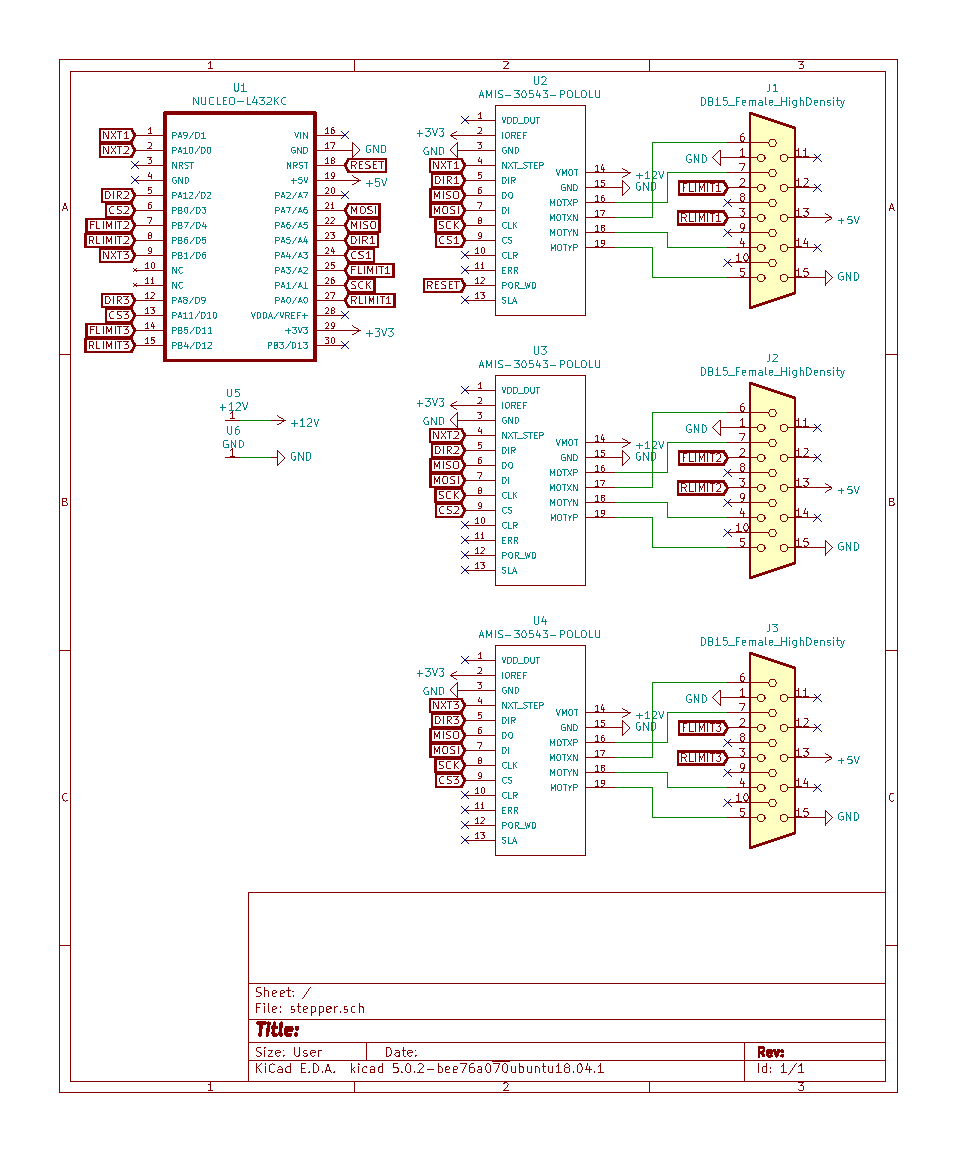
\includegraphics[width = \textwidth]{schematics.pdf}
\caption {Schematics of the LUMS stepper.} \label{schematics}
\end{figure}


\begin{figure}[h]
 \centering
 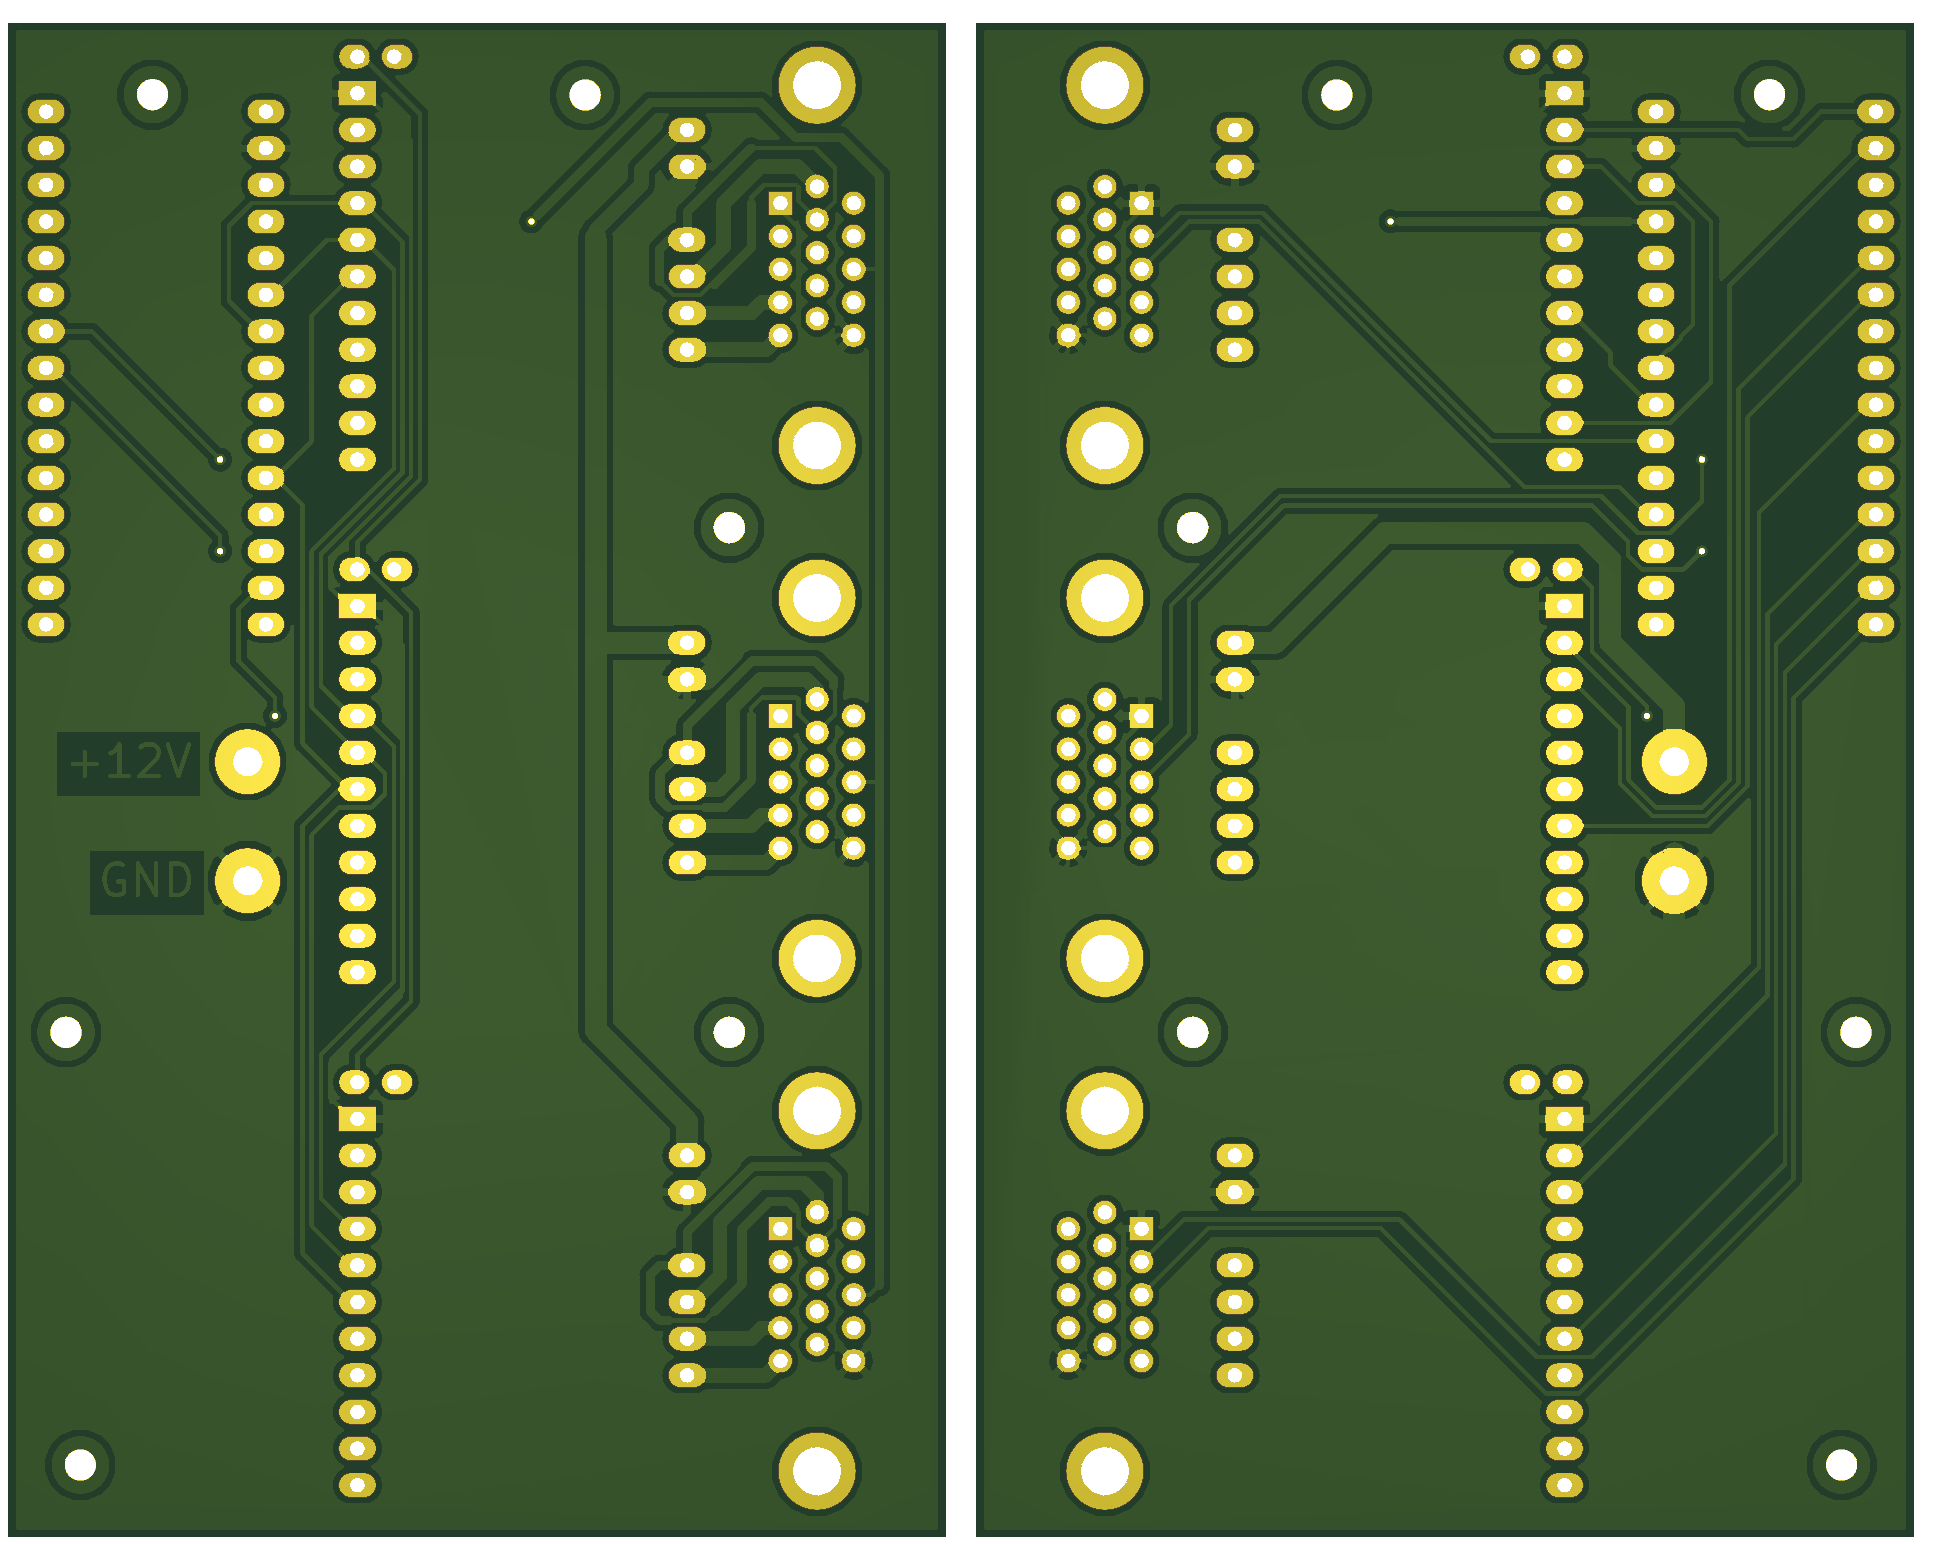
\includegraphics[width = 14cm]{render.png}
\caption {PCB design. View from top and bottom, respectively.} \label{pcb}
\end{figure}

\begin{figure}[h]
 \centering
 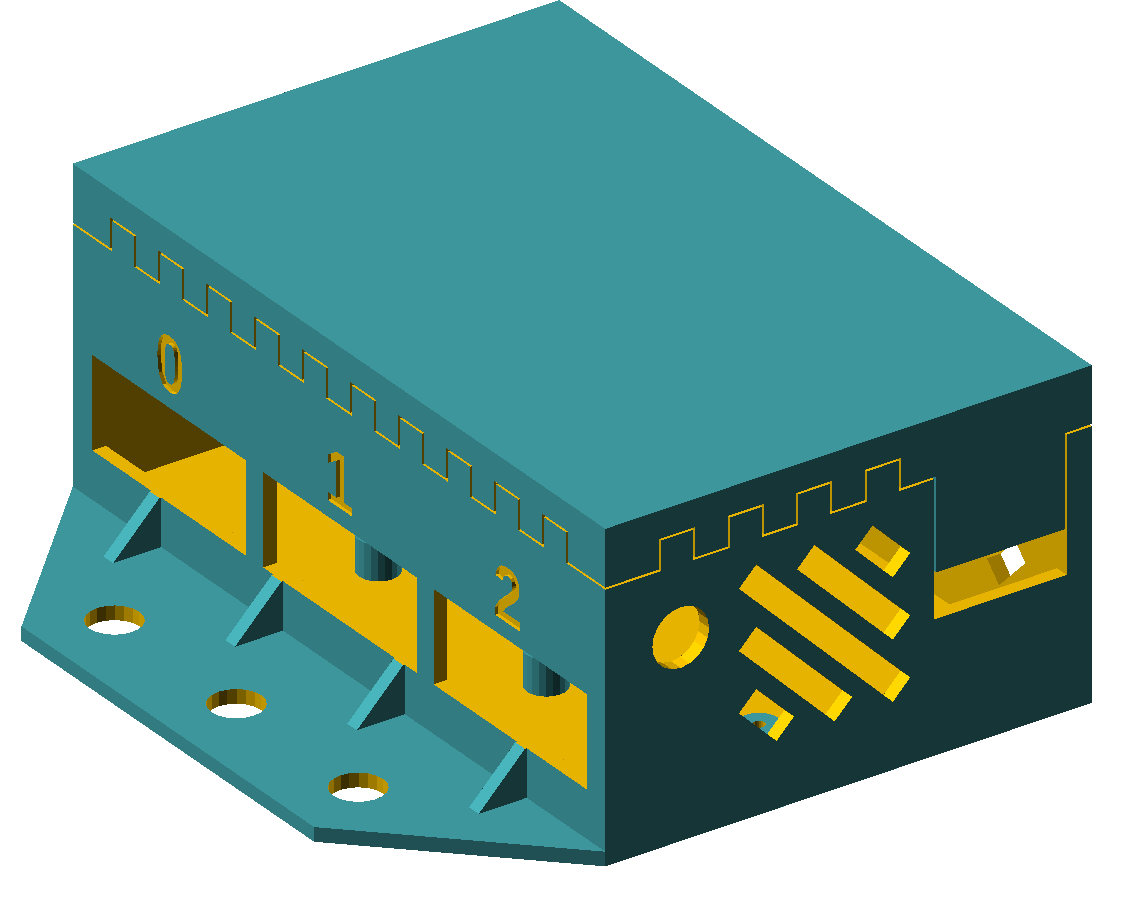
\includegraphics[width = 15cm]{case.png}
\caption {Case, model for 3D printer.} \label{case}
\end{figure}




%\begin{thebibliography}{99}
%\bibitem{Kopp} Arnold Kopp et. al. Natura 6 (2018)
%\end{thebibliography}

\end{document}












\grid
